
%(BEGIN_QUESTION)
% Copyright 2007, Tony R. Kuphaldt, released under the Creative Commons Attribution License (v 1.0)
% This means you may do almost anything with this work of mine, so long as you give me proper credit

Industrial operations using large quantities of steam often distribute it at different pressures, much like an electrical utility system distributing power at several different voltages:

$$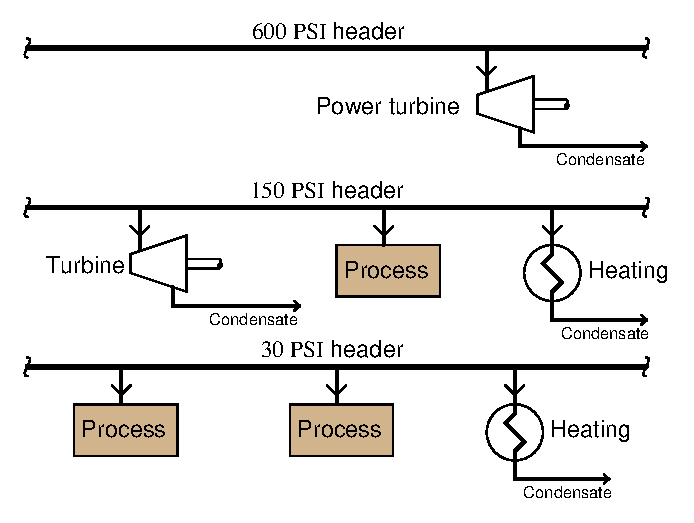
\includegraphics[width=15.5cm]{i01801x01.eps}$$

It may not always be practical to have a separate boiler (or set of boilers) for each header pressure (e.g. one boiler outputting 600 PSI, one outputting 150 PSI, and one outputting 30 PSI).  So, often there is a need to ``let down'' high-pressure steam to a lower pressure.

Although it is possible to simply use control valves to throttle high-pressure steam into a lower-pressure headers, this would be a waste of energy.  Such a strategy would be analogous to using resistive voltage dividers to step high voltage down to lower values in an electric power system:

$$\includegraphics[width=15.5cm]{i01801x02.eps}$$

An improvement over the plain let-down strategy is to use special {\it desuperheating} valves instead of normal throttling valves.  Desuperheating is a process whereby water is sprayed into the throttled steam:

$$\includegraphics[width=15.5cm]{i01801x03.eps}$$

Desuperheaters may be thought of as the steam equivalent of electrical transformers: a much more efficient means of reducing pressure (voltage) than throttling with a restrictive (resistive) element.  Explain how desuperheating works, and why the electrical transformer analogy is appropriate.

\underbar{file i01801}
%(END_QUESTION)





%(BEGIN_ANSWER)

The water injected in a desuperheating valve gains heat energy from the superheated let-down steam, producing a greater volume of steam at a lower pressure (and lower temperature), much like an electrical transformer steps down voltage with a corresponding {\it increase} in current.  Desuperheaters exchange temperature for volume, much like transformers exchange voltage for current (or vice-versa).

\vskip 10pt

Challenge question: explain why turbines make efficient steam pressure let-down devices:

$$\includegraphics[width=15.5cm]{i01801x04.eps}$$

%(END_ANSWER)





%(BEGIN_NOTES)


%INDEX% Physics, heat and temperature: desuperheating
%INDEX% Physics, heat and temperature: superheated steam

%(END_NOTES)


